Postupně jsme testovali čtyři vzorky rezistorů a to konkrétně jejich výkonovou zatížitelnost v závislosti na použitém substrátu. Na laboratorním zdroji (TTi QPX1200SP) jsme nastavili napětí \qty{7}{V} a přibližně odečetli také odebíraný proud, pro všechny vzorky to bylo \qty{0,06}{A}. Vzorky pokryté termoemisní barvou jsme následně pozorovali termokamerou (FLUKE) a po ustálení stavu, tedy při maximální dosažené teplotě, jsme hodnoty zaznamenali. Porovnání jednotlivých měření se nachází na Obr.~\ref{fig:termo-png}.

\begin{figure}[h!]
    \centering
    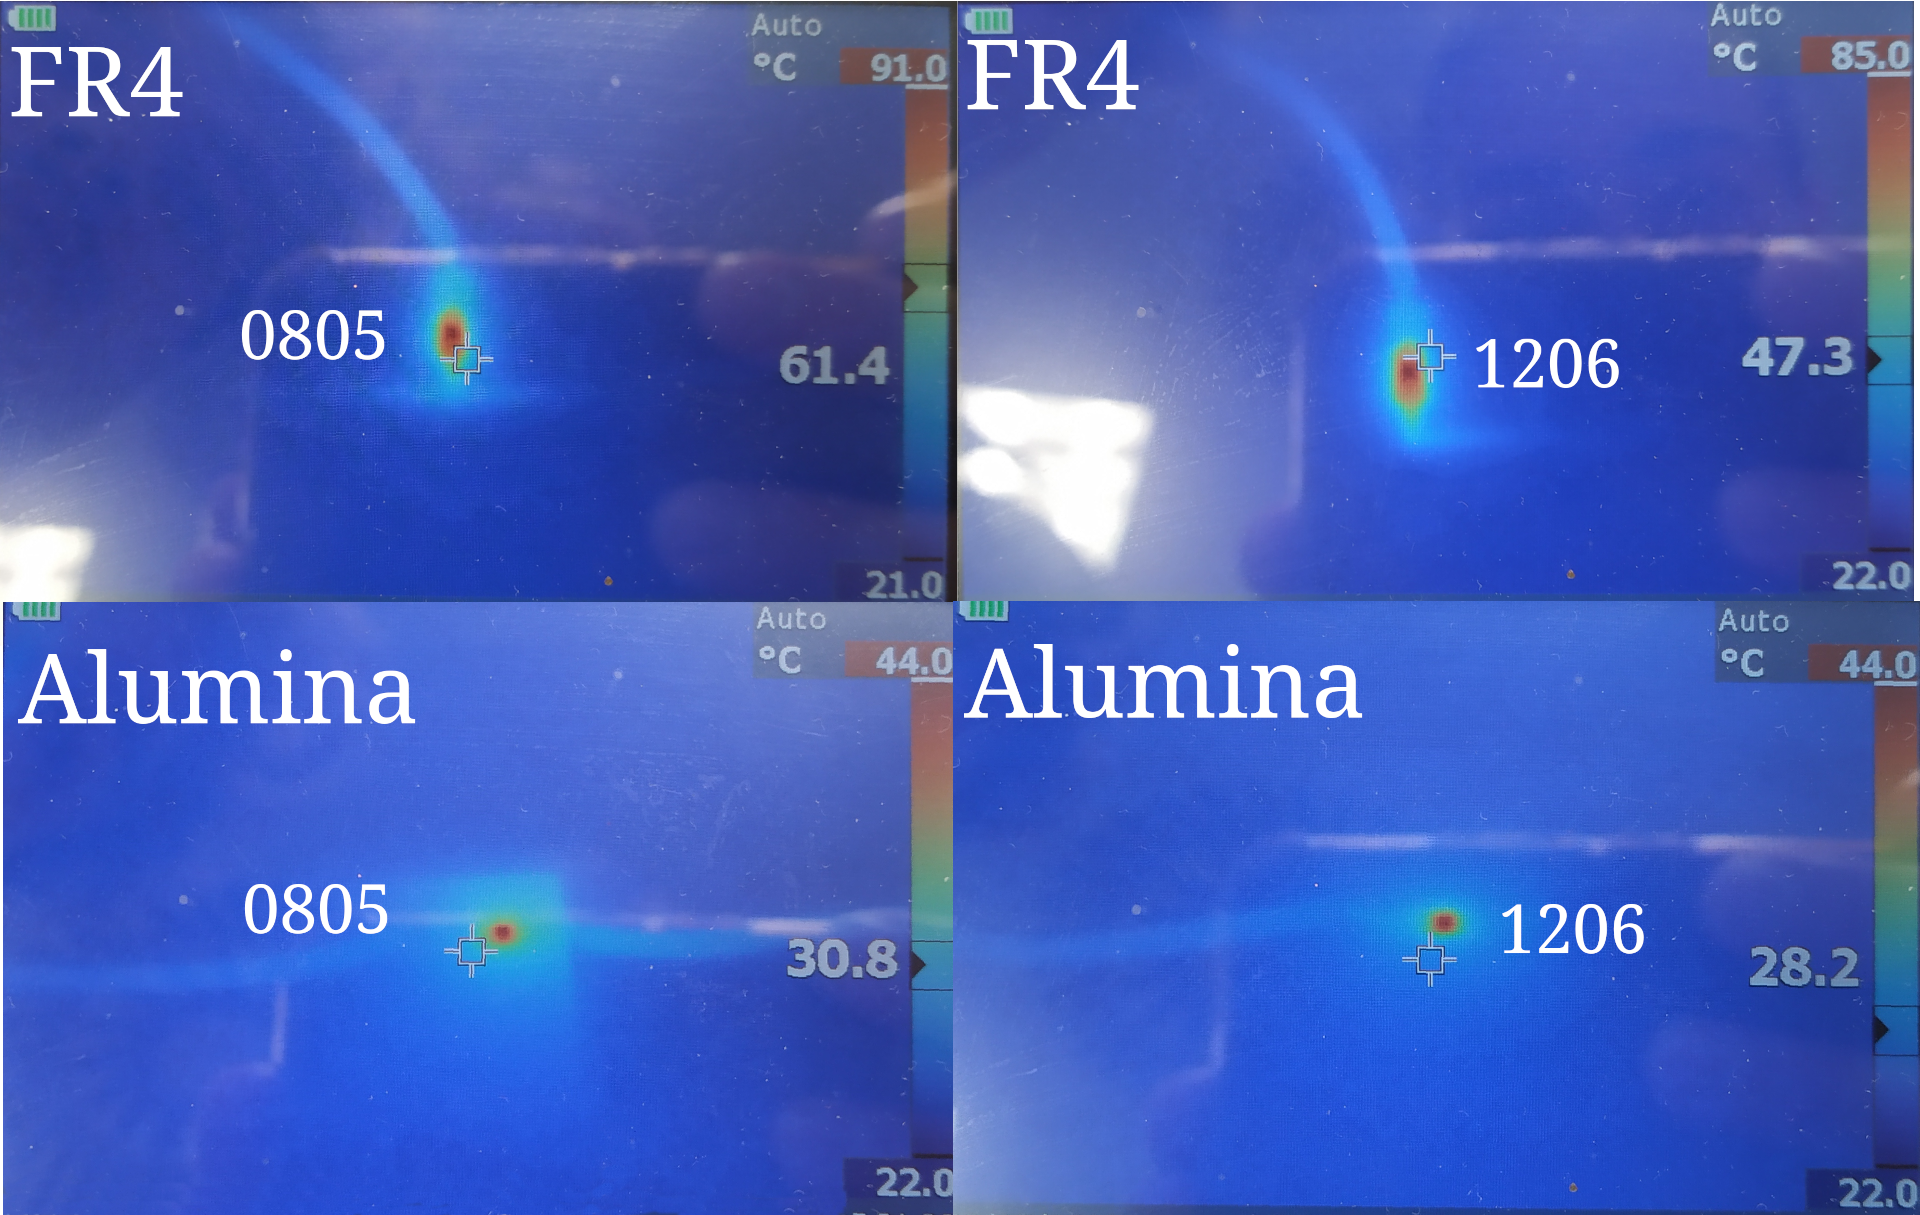
\includegraphics[width=0.8\textwidth]{termo.png}
    \caption{Porovnání ohřevu SMD rezistorů pouzder 0805 a 1206 na různých substrátech.}
    \label{fig:termo-png}
\end{figure}

Ve druhé části byl proveden destruktivní test SMD rezistoru. Zvyšováním napětí na laboratorním zdroji dochází k nárustu procházejícího proudu, ohřevu rezistoru a následně tepelnému poškození a zničení celé součástky. Výsledek testu je zobrazen na Obr.~\ref{fig:destrukce-png}. Průbeh zkoušky popisuje Tab.~\ref{tab:popis_destrukce}.

\begin{table}[h!]
    \caption{Průběh destruktivního testu SMD rezistoru.}
    \centering
    \def\arraystretch{1.4}
    \begin{tabular}{l|l}
        U\ [V] &  Popis situace \\ \hline  \hline
            12,5 &  rezistor syčí \\ \hline
            14,3 &  odpařování tavidla \\ \hline
            22,2 &  nečitelný popisek \\ \hline
            24,7 &  zvýšený zápach \\    \hline
            25,6 &  viditelné žhavé místo \\ \hline
            26,9 &   spálení součástky \\ 
    \end{tabular}
    \label{tab:popis_destrukce}
\end{table}


\begin{figure}[h!]
    \centering
    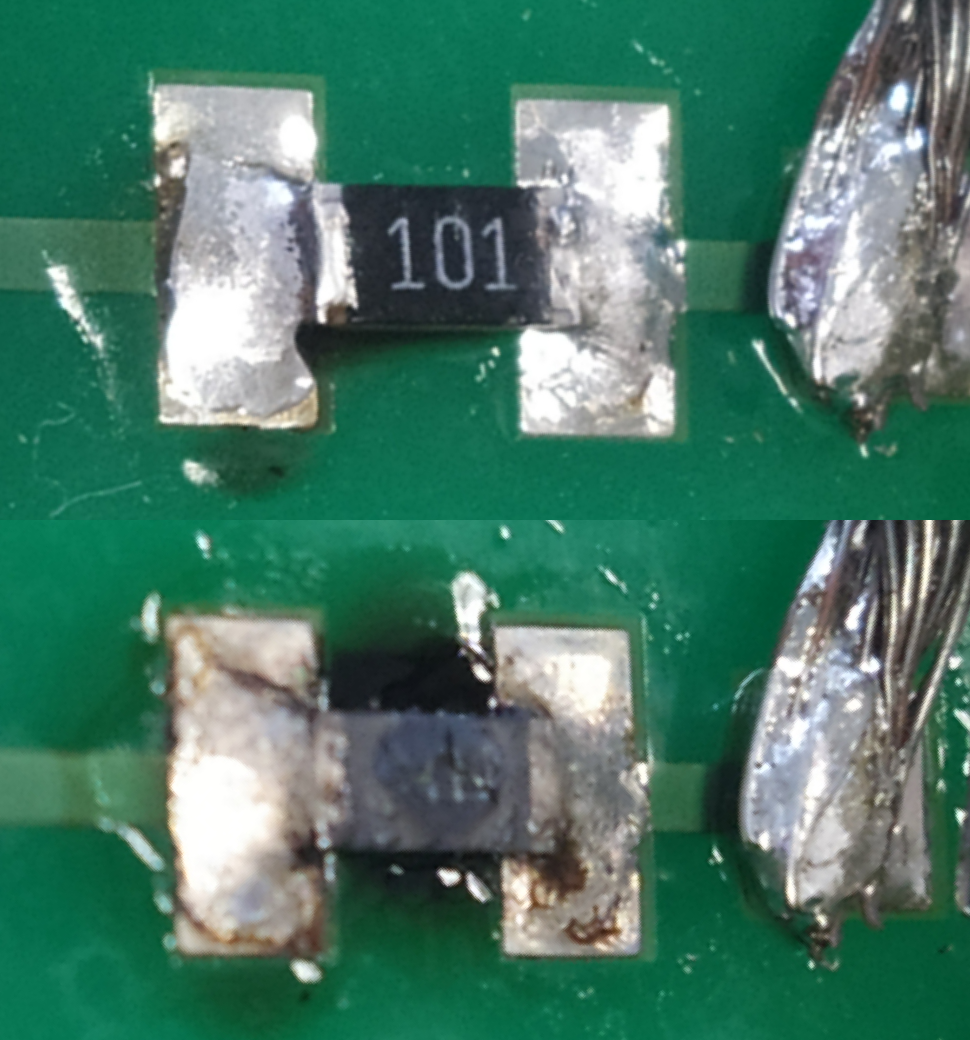
\includegraphics[width=0.8\textwidth]{destrukce.png}
    \caption{Destrukční test SMD rezistoru.}
    \label{fig:destrukce-png}
\end{figure}

